\documentclass[a4paper]{scrreprt}
\usepackage{fancyhdr}
\pagestyle{fancy}
\usepackage[english]{babel}
\usepackage[utf8]{inputenc}
\usepackage{graphicx}
\usepackage{url}
\usepackage{textcomp}
\usepackage{amsmath}
\usepackage{lastpage}
\usepackage{pgf}
\usepackage{wrapfig}
\usepackage{fancyvrb}
\usepackage{appendix}
\usepackage{pdfpages}
\usepackage{xcolor}
\usepackage{hyperref}
\usepackage{placeins}

\hypersetup{
    colorlinks=true,
    linkcolor=blue,
    filecolor=black,      
    urlcolor=blue,
    citecolor=black,
}

% Create header and footer
\headheight 27pt
\pagestyle{fancyplain}
\lhead{\footnotesize{Datalagring, IV1351}}
\chead{\footnotesize{Task 3}}
\rhead{}
\lfoot{}
\cfoot{\thepage\ (\pageref{LastPage})}
\rfoot{}

% Create title page
\title{Task 3, version 2}
\subtitle{Datalagring, IV1351}
\author{Adrian Jonsson Sjödin \\ adriansj@kth.se}
\date{\today} 


\begin{document}

\maketitle

\tableofcontents %Generates the TOC

\chapter{Introduction}
The purpose of task 3 was to write OLAP queries towards the database created in task 2, and confirm that everything works as intended. The creation and reasoning behind 
the OLAP queries is what will be covered in this report.

\chapter{Method}
The DBMS used for the Sound Good Music School database is MySQL 8 and the queries was developed using a combination of MySQL Workbench and the CLI. 

The process behind creating the queries was to first breaking them up into smaller parts and test that we got the expected output from them when they where run in the CLI, and then 
keep building upon them until we achieve the sought after query. For this we used MySQL Workbench since it is easier to write the code and modify it there than directly in the CLI.

The queries was then tested manually by retrieving the data in question from the right tables and manually look at the tables and see if the query result matched what we got when we looked directly at the tables 
and noted with pen and paper the data. 


\chapter{Result}
\label{sec:result}
The SQL scripts can be found here:
 \href{https://github.com/adrian-jonsson-sjoedin/IV1351-Datalagring/tree/main/project/SQL}{GitHub}.


\begin{figure}[h]
    \begin{center}
        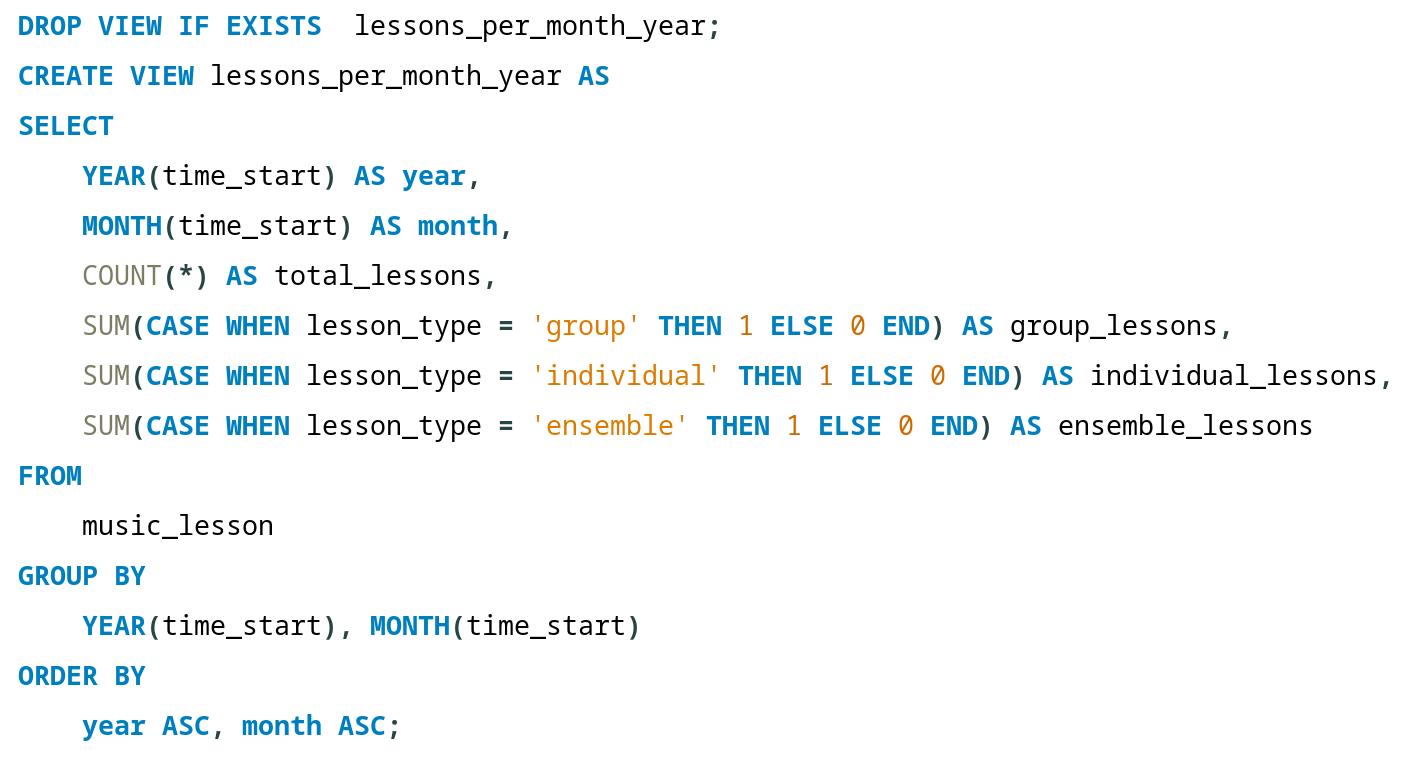
\includegraphics[width=0.70\textwidth]{../img/lessonSQLv2.png} \\
        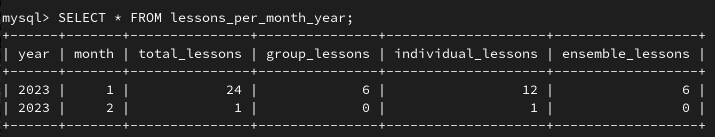
\includegraphics[width=0.70\textwidth]{../img/lessonV2.png}
        \caption{Total number of lessons per year and month for each lesson type}
        \label{fig:lessons}
    \end{center}
\end{figure}
\begin{figure}[h]
    \begin{center}
        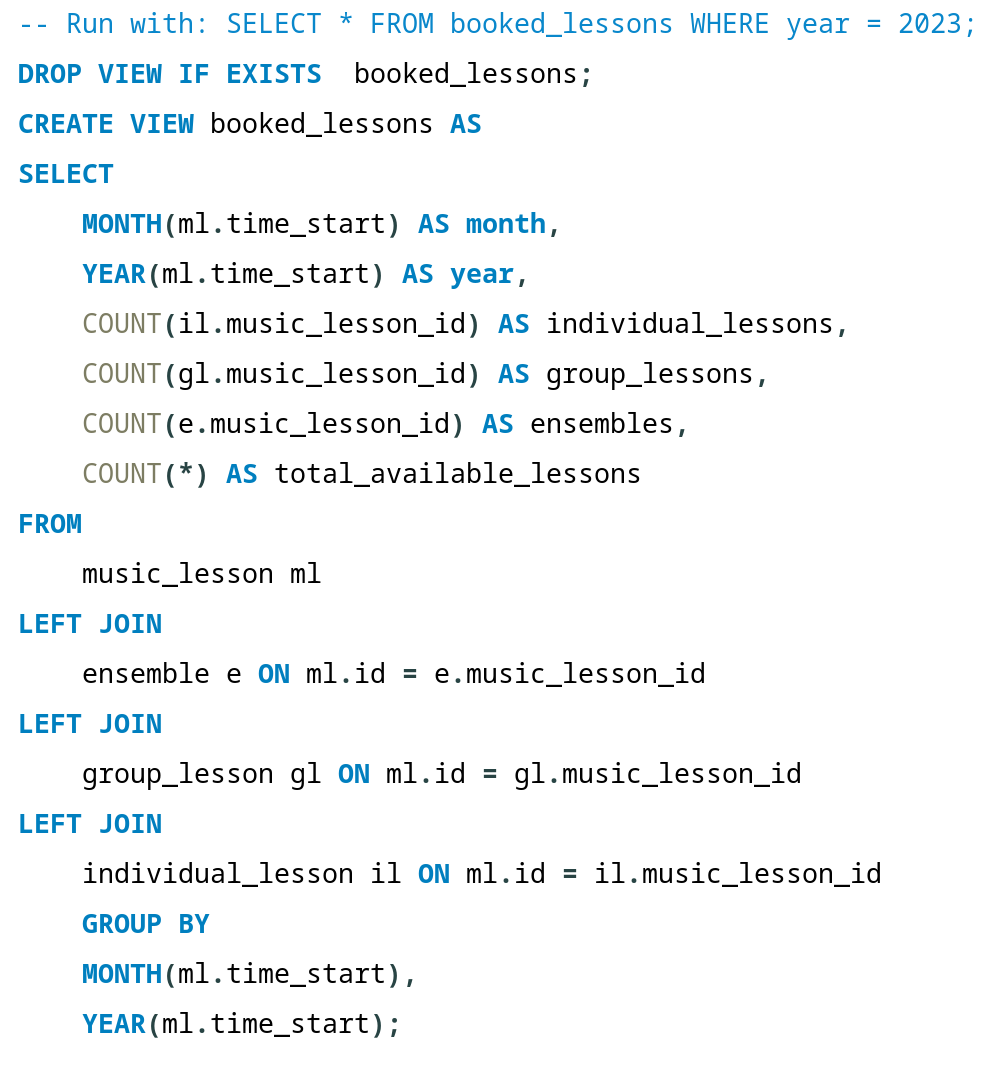
\includegraphics[width=0.70\textwidth]{../img/bookedLessonSQL.png} \\
        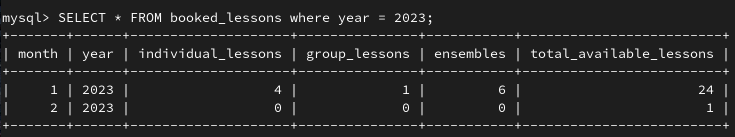
\includegraphics[width=0.70\textwidth]{../img/bookedLessons.png}
        \caption{Total number of available lesson per year and month and how many lessons have students that have booked them for each lesson type}
        \label{fig:booked}
    \end{center}
\end{figure}
\begin{figure}[h]
    \begin{center}
        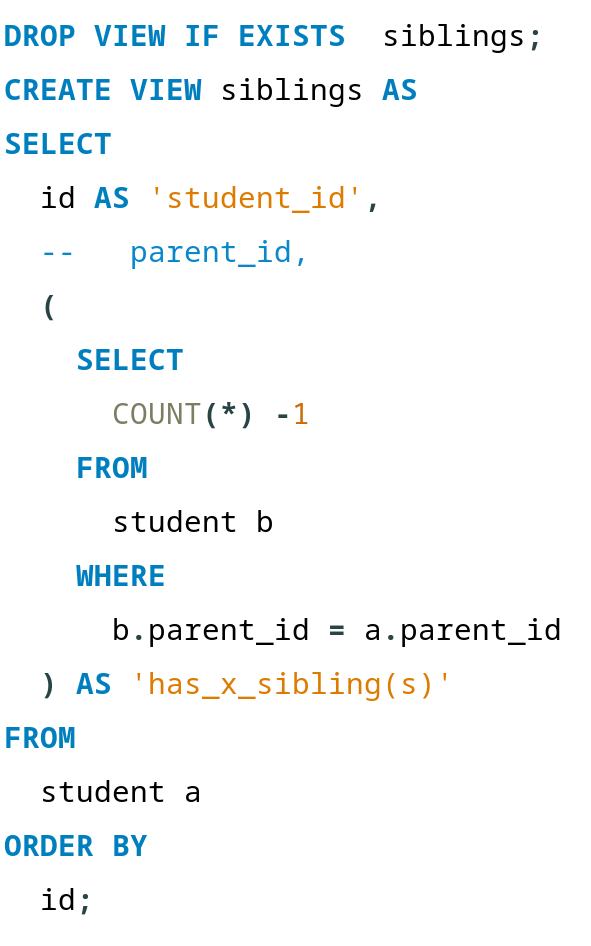
\includegraphics[width=0.49\textwidth]{../img/siblingsSQLv2.png} 
        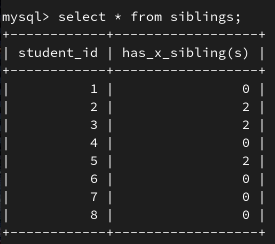
\includegraphics[width=0.49\textwidth]{../img/siblingsV2.png}
        \caption{The number of siblings for each student}
        \label{fig:siblings}
    \end{center}
\end{figure}
\begin{figure}[h]
    \begin{center}
        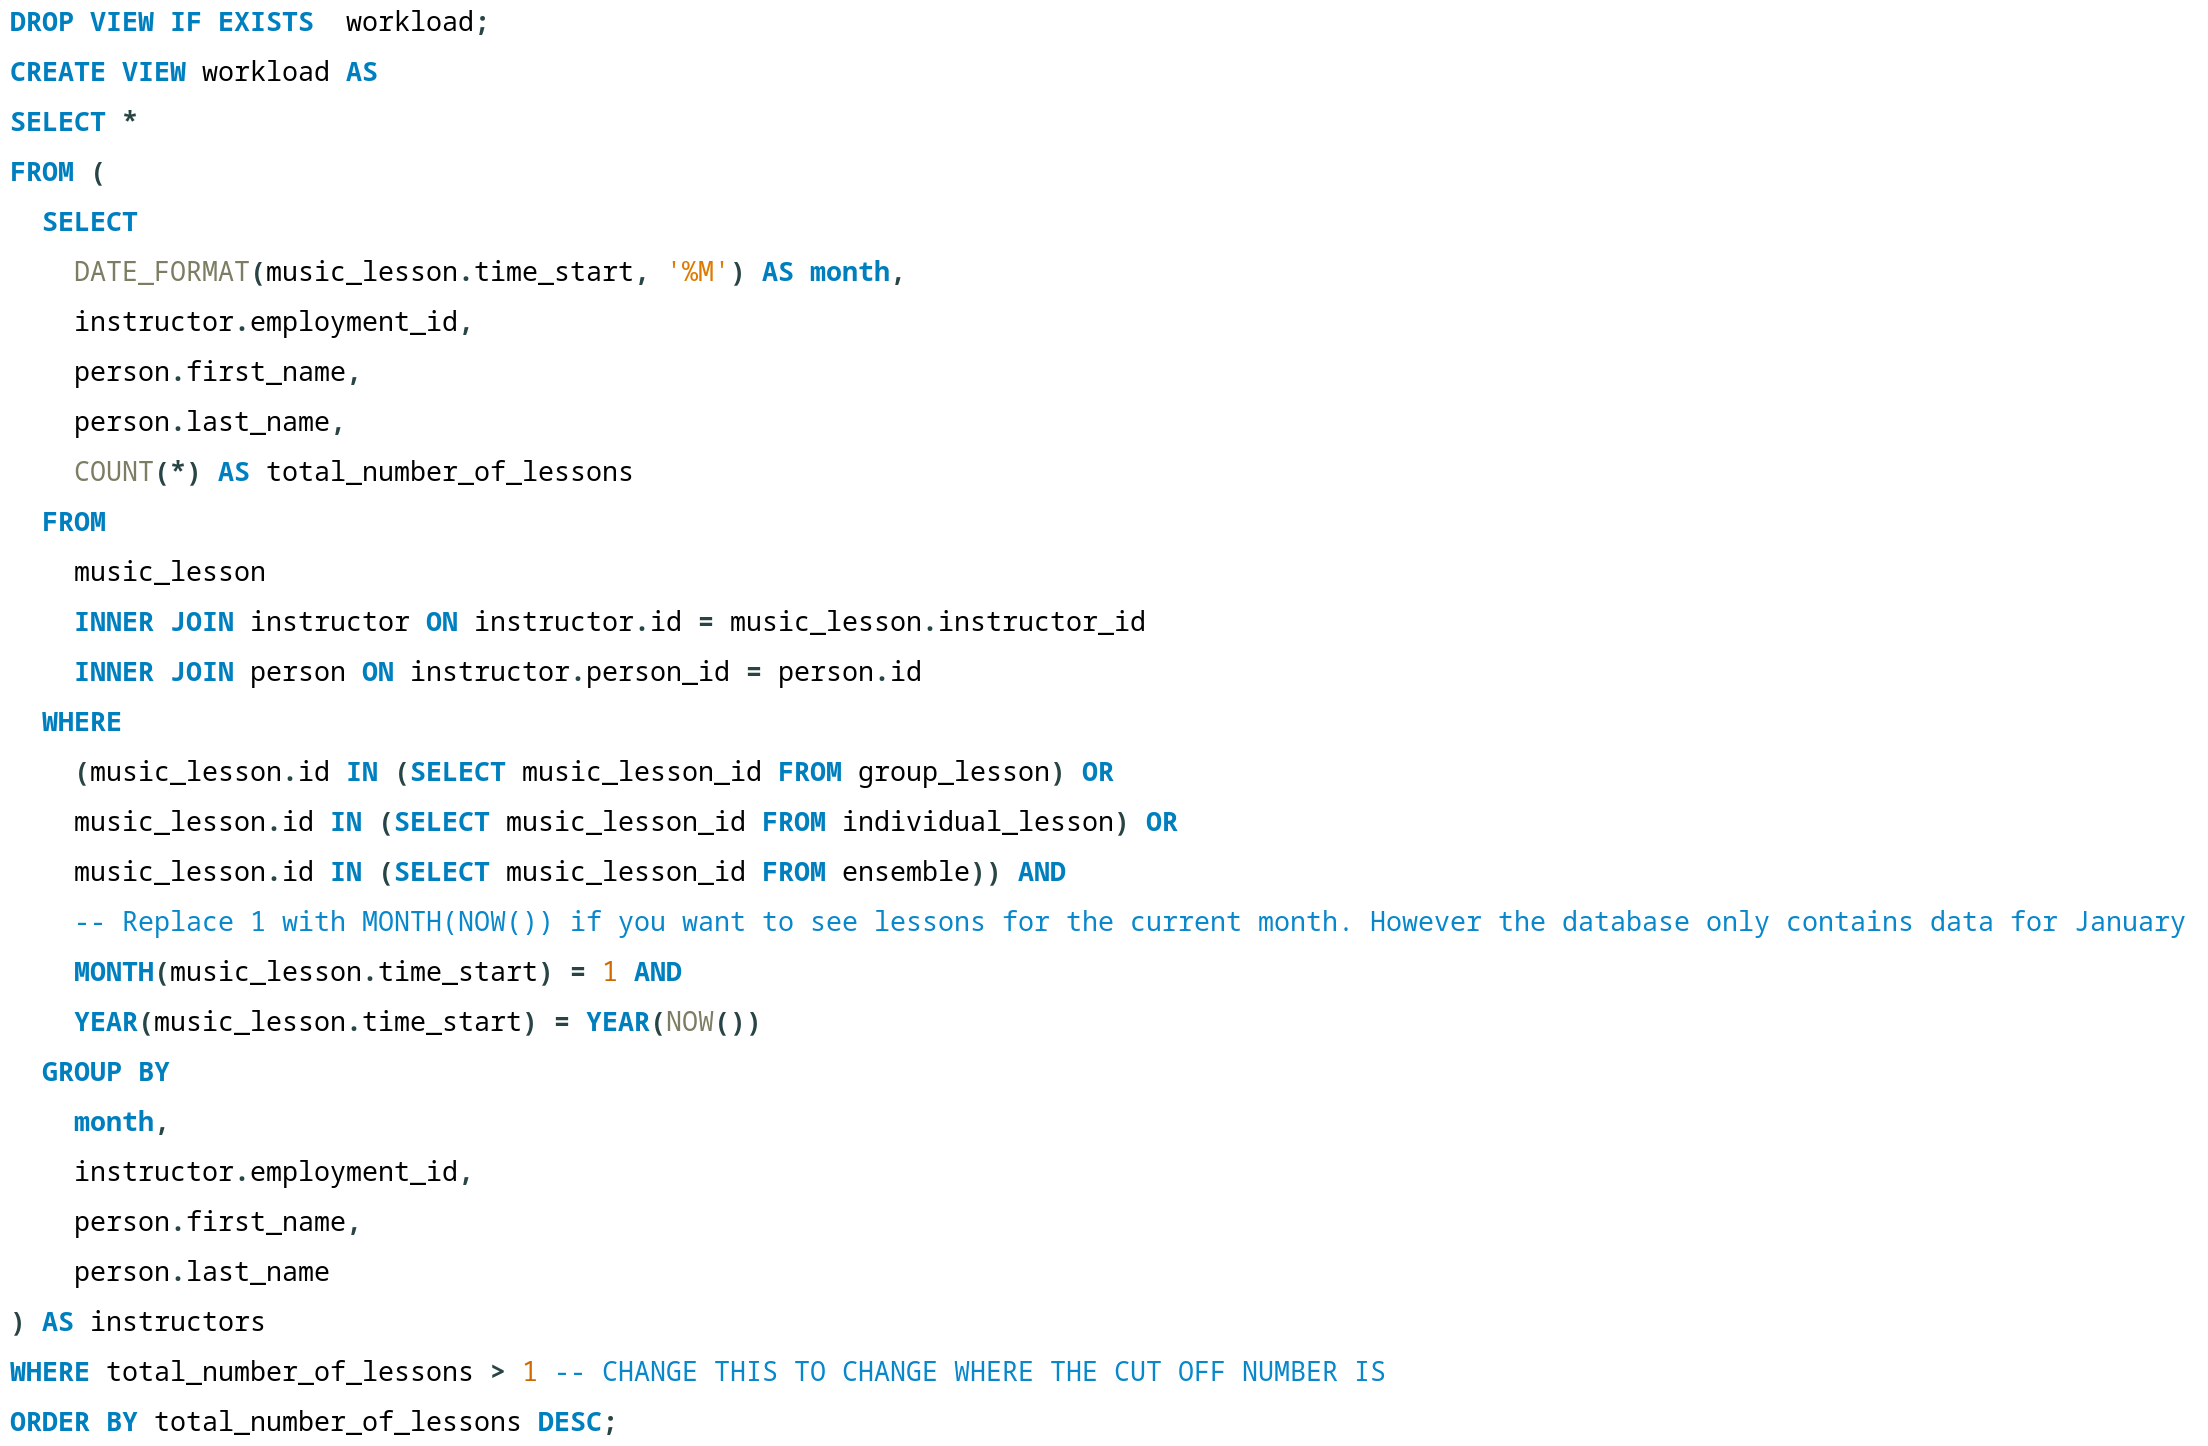
\includegraphics[width=\textwidth]{../img/workloadSQLv2.png} \\
        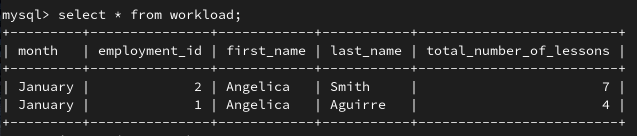
\includegraphics[width=0.76\textwidth]{../img/workloadV2.png}
        \caption{List of all instructors that have more than a specific nr of lesson \\during the current month}
        \label{fig:workload}
    \end{center}
\end{figure}
\begin{figure}[h]
    \begin{center}
        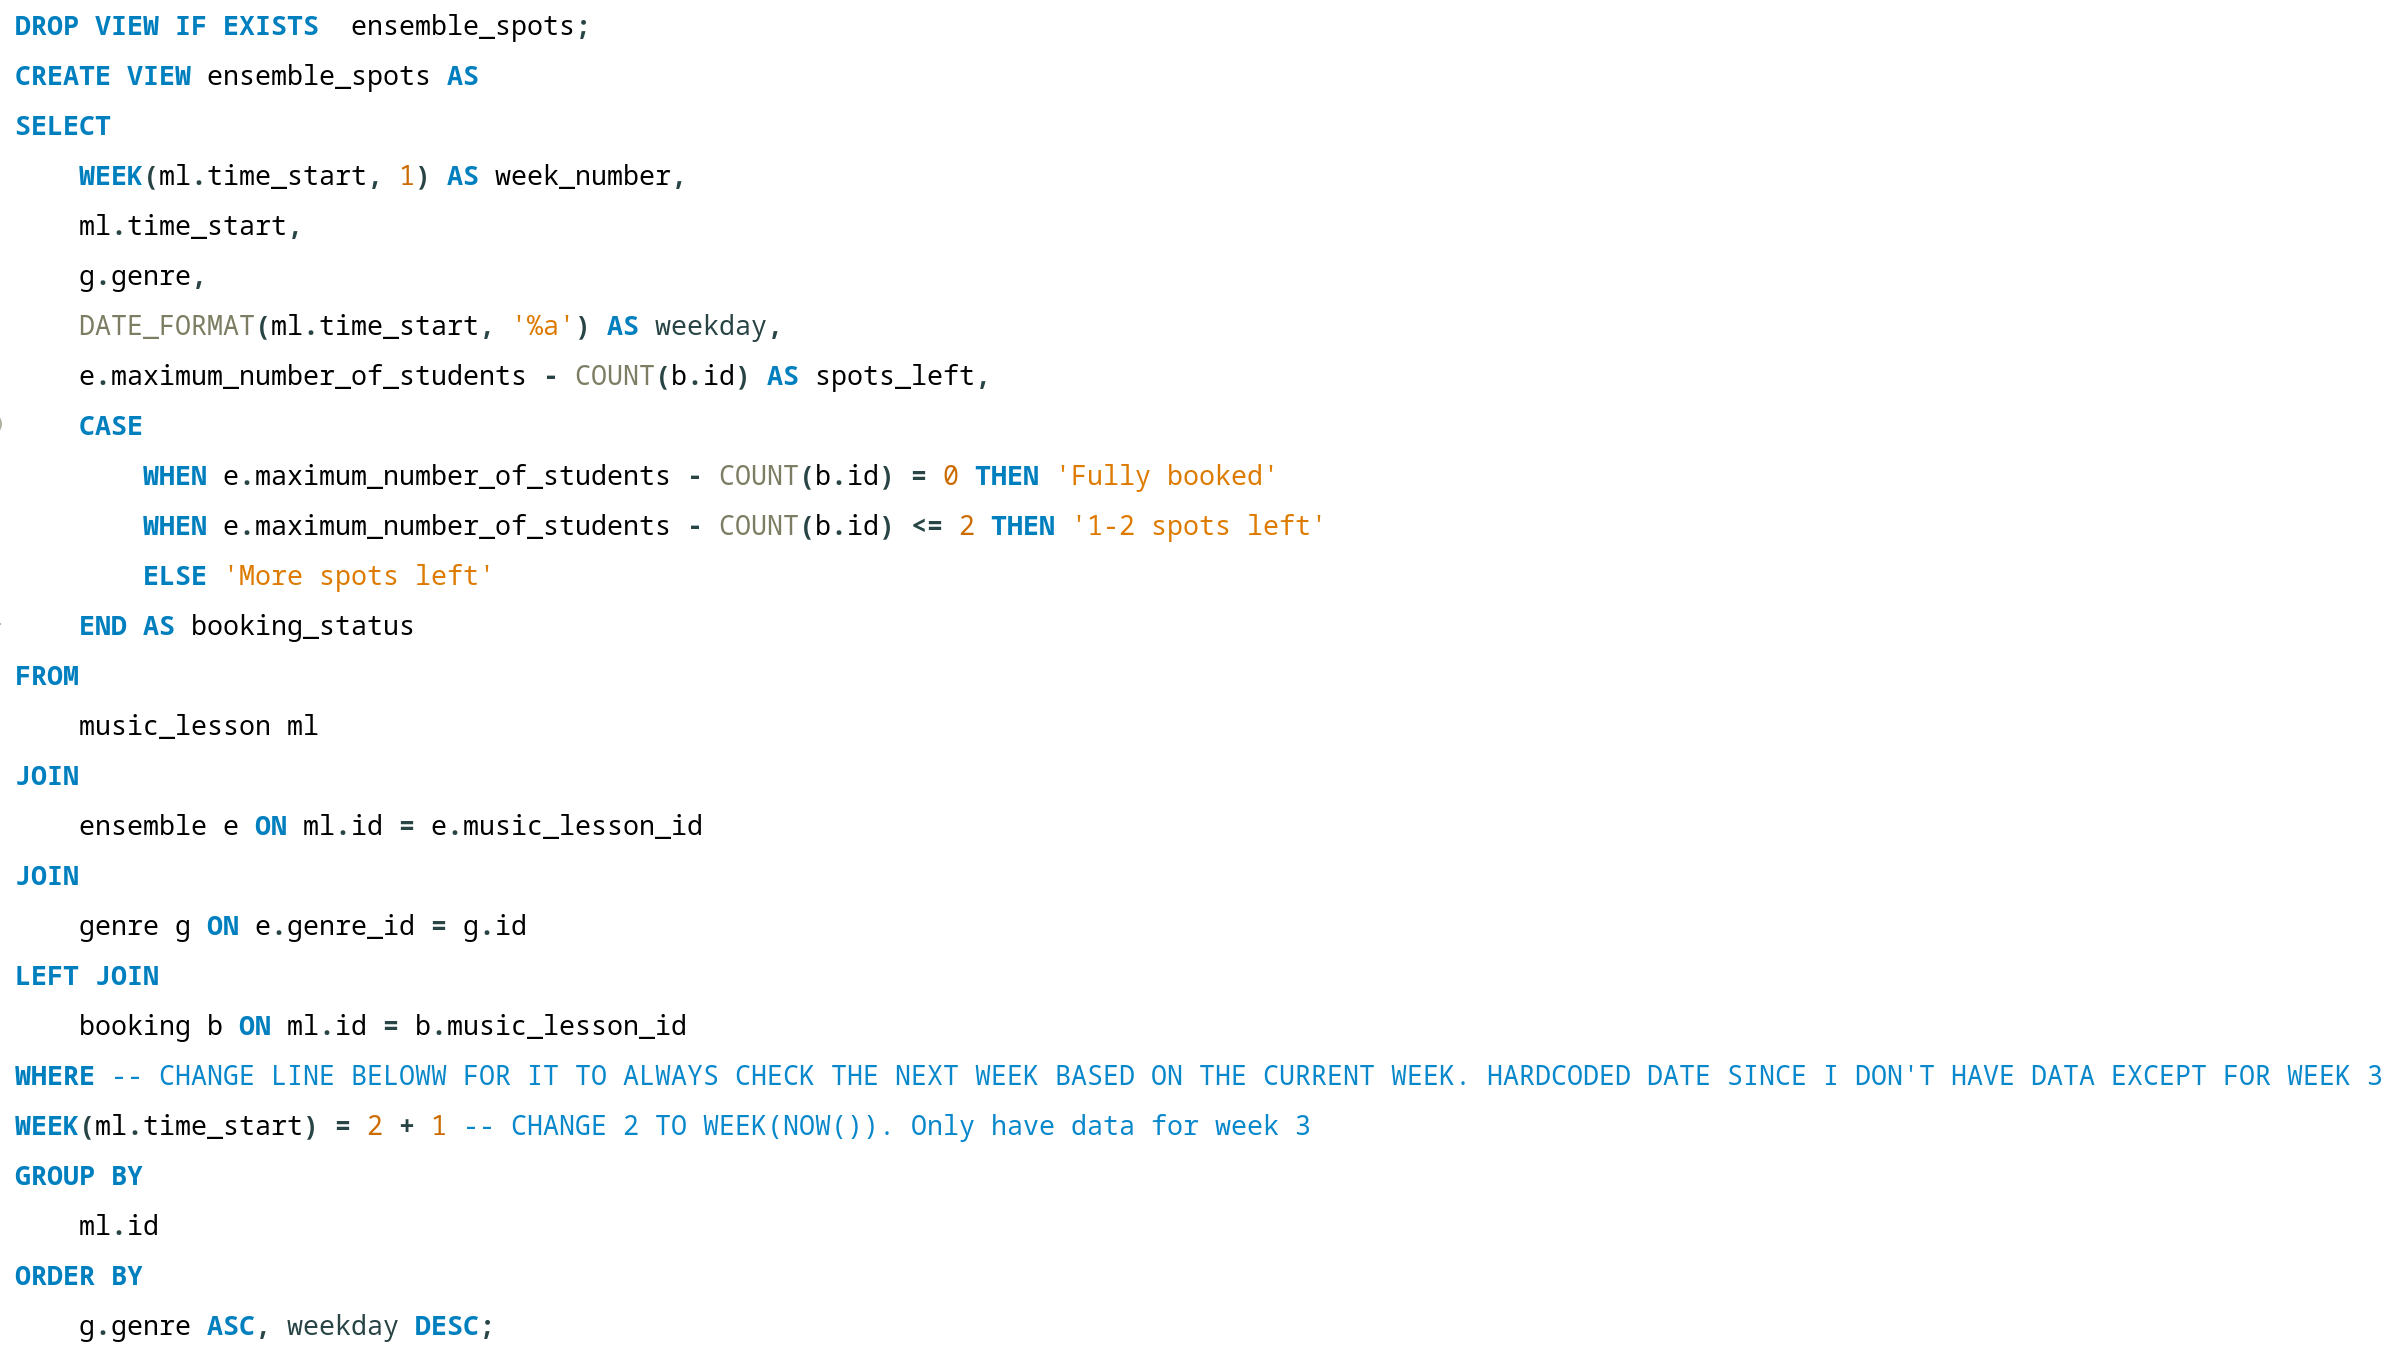
\includegraphics[width=\textwidth]{../img/ensembleSQLv2.png} \\
        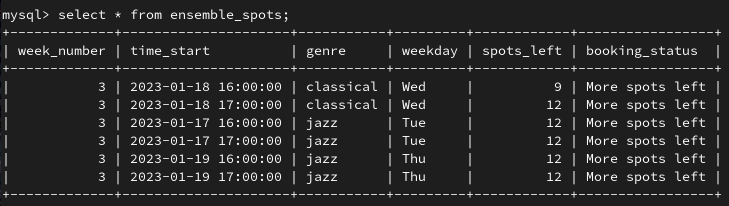
\includegraphics[width=\textwidth]{../img/ensembleSpotsV2.png}
        \caption{List all ensembles held during the next week and how many spots are left, sorted by music genre and weekday}
        \label{fig:ensemble}
    \end{center}
\end{figure}
\begin{figure}[h]
    \begin{center}
        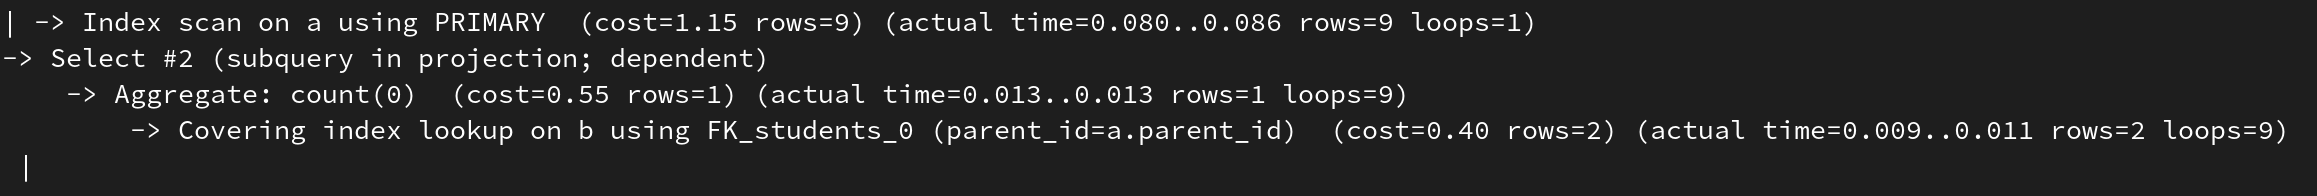
\includegraphics[width=\textwidth]{../img/explain_no_view_siblings.png} \\
        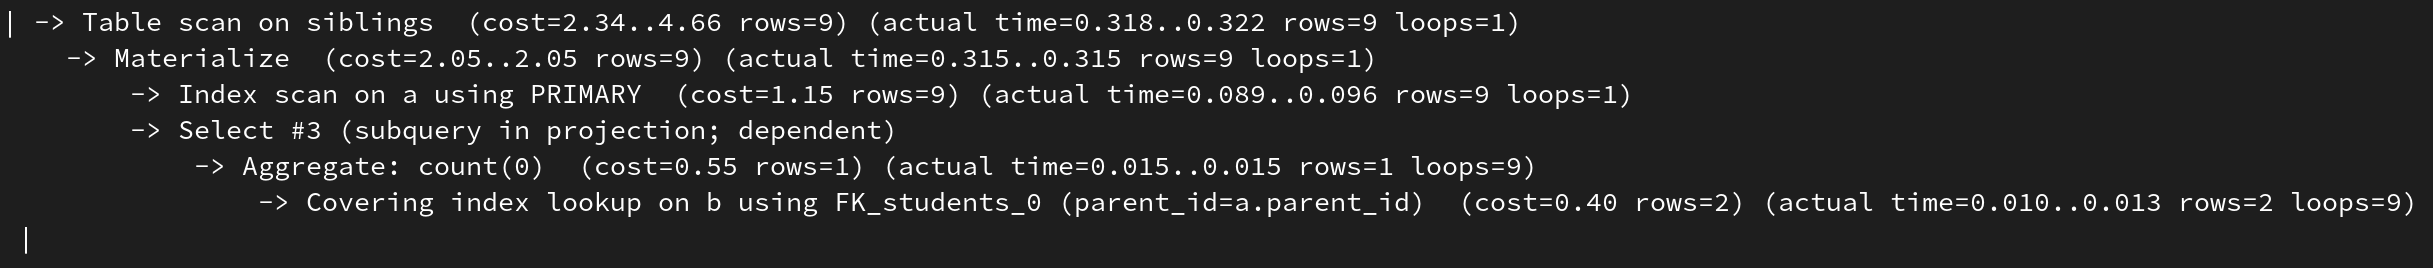
\includegraphics[width=\textwidth]{../img/explain_sibling.png}
        \caption{On top is the query from fig. \ref{fig:siblings} without storing it in a view while the bottom is the same query when stored in a view}
        \label{fig:explainSiblings}
    \end{center}
\end{figure}

The query seen in fig. \ref{fig:lessons} is the one that gives how many lectures we have per month and year and how many of each type. The leftmost column in it tells us how many 
available lessons the school currently have by looking in the "music\_lesson" table. The other three columns shows us how many of each type we have. It is the easiest query out of 
the four and uses aggregate functions in combination with flow control functions.

In fig. \ref{fig:booked} we have a similar query but in this one the three columns that correspond to the different lesson types instead tells us how many of that type have been created. They will only 
be created when a new booking is created for a student to a lesson and thus tells us how many of the different lessons have at least one student signed up to it. This query uses aggregate functions and 
JOIN operators.


The query seen in fig. \ref{fig:siblings} is the one that displays how many siblings each student have that is also enrolled at the school. This query uses a correlated sub-query to achieve the sought after 
result.

The query seen in fig. \ref{fig:workload} is the one that list all instructors that have more than a specific number of lessons during the current month. This and the next query were the ones who gave me the most 
trouble. This because the query makes use of sub-queries, JOIN clauses, aggregate functions, and conditional filtering, making it quite complex for me. 
Note that the column "total\_number\_of\_lessons" is counting just the lessons that have students assign to them. I did it this way because it felt the most relevant to know because if there's no students 
taking a class it stands to reason that the instructor won't be holding that class. If one want to get just the total number of lessons an instructor is assigned to then one can easily get that from the 
"music\_lesson" table.

Lastly we have the query seen in fig. \ref{fig:ensemble} which is the one that lists all available ensemble spots for the coming week. Like the previous query it utilizes a combination JOIN clauses, 
aggregate functions, flow control functions, conditional filtering with the WHERE clause, and GROUP BY and ORDER BY clauses for grouping and sorting the results.

In the last figure \ref{fig:explainSiblings} we see the result of running \textbf{EXPLAIN ANALYZE} on the query \ref{fig:siblings}.




\chapter{Discussion}
As can be seen from the queries in the Result section, all queries are stored as views. This is to make it easier to run them at a later date. All queries except the 
query seen in fig. \ref{fig:booked} are stored in full. This was done because only that query had the requirement of being able to vary what was shown based of a 
requirement. The rest of them didn't have that condition and thus it would be easier to store the whole query as a view. 

The reason why I didn't use materialized view is simply because MySQL 8 (or earlier versions) doesn't support it. If I could have used them then I would most 
likely have used them on query \ref{fig:lessons}, \ref{fig:siblings} and \ref{fig:workload}. 

The first since the query is expected to be performed a few times per week and involves aggregation. Furthermore the rows in the table "music\_lesson" will most likely be created in 
batches as the schedule is set and thus the view shouldn't need to be updated that often. This would allow for a faster reading of data whenever it is needed, with the drawback of having to update the 
table whenever new lessons are added. But most likely that wouldn't be too often making it worthwhile turning it into a materialized view.


While the query seen in fig. \ref{fig:siblings} is simple I would still turn it into a materialized view since there will most likely be a significant larger number of times that I will read the table,
as opposed to updating it. After all it will only be required to be updated whenever a new student have been added to check if said student has a sibling already enrolled in the school.

Lastly the query seen in fig. \ref{fig:workload} would probably benefit from being a materialized view as the query is expected to be executed daily and involves multiple joins and aggregation functions.

For the rest of the queries I think a view is the better choice since the columns containing the data we need to retrieve most likely will be updated often. For example 
the result from query \ref{fig:ensemble} will change whenever another students booking for an ensemble lessons is accepted, or they cancel their booking. And since the 
result will be displayed on the web page it needs to be up to date.

The database didn't need any permanent changes to make the queries. I did however have to insert some extra data to test some of the queries since I've only inputted lesson for a few days in the database. 


We see in \ref{fig:explainSiblings} a slight difference between the two results. When run on the saved view, MySQL first materialize the view, which means it creates a temporary table containing 
the result of the view, and then scans that temporary table. On the other hand when \textbf{EXPLAIN ANALYZE} is run on the original query MySQL directly executes the query without materializing it first.
The actual execution time and other metrics however are very similar between the two results, with only small minor differences. The most time-consuming part of the query is as expected 
the correlated sub-query. This sub-query is executed once for each row returned by the outer query, as is indicated by the loops=9 in both cases.

One way of optimizing the query could be by trying to use a derived table with a \textbf{JOIN} instead of the correlated sub-query. That way one could avoid executing the sub-query multiple times which may 
lead to better performance. However I didn't manage to implement it different earlier and because of time constraints it will have to stay as a correlated sub-query unfortunately.

\end{document}
